%You can leave alone everything before Line 79.
\documentclass{article}
\usepackage{url,amsfonts, amsmath, amssymb, amsthm,color, enumerate, verbatim}
% Page layout
\setlength{\textheight}{8.75in}
\setlength{\columnsep}{2.0pc}
\setlength{\textwidth}{6.5in}
\setlength{\topmargin}{0in}
\setlength{\headheight}{0.0in}
\setlength{\headsep}{0.0in}
\setlength{\oddsidemargin}{0in}
\setlength{\evensidemargin}{0in}
\setlength{\parindent}{1pc}
\newcommand{\shortbar}{\begin{center}\rule{5ex}{0.1pt}\end{center}}
%\renewcommand{\baselinestretch}{1.1}
% Macros for course info
\newcommand{\courseNumber}{ME 552}
\newcommand{\courseTitle}{Mechatronics}
\newcommand{\semester}{Fall 2012}
\newcommand{\xxx}[1]{\textcolor{red}{#1}}
% Theorem-like structures are numbered within SECTION units
\theoremstyle{plain}
\newtheorem{theorem}{Theorem}[section]
\newtheorem{lemma}[theorem]{Lemma}
\newtheorem{corollary}[theorem]{Corollary}
\newtheorem{proposition}[theorem]{Proposition}
\newtheorem{statement}[theorem]{Statement}
\newtheorem{conjecture}[theorem]{Conjecture}
\newtheorem{fact}{Fact}
%definition style
\theoremstyle{definition}
\newtheorem{definition}[theorem]{Definition}
\newtheorem{example}{Example}
\newtheorem{problem}[theorem]{Problem}
\newtheorem{exercise}{Exercise}
\newtheorem{algorithm}{Algorithm}
%remark style
\theoremstyle{remark}
\newtheorem{remark}[theorem]{Remark}
\newtheorem{reduction}[theorem]{Reduction}
%\newtheorem{question}[theorem]{Question}
\newtheorem{question}{Question}
%\newtheorem{claim}[theorem]{Claim}
%
% Proof-making commands and environments
\newcommand{\beginproof}{\medskip\noindent{\bf Proof.~}}
\newcommand{\beginproofof}[1]{\medskip\noindent{\bf Proof of #1.~}}
\newcommand{\finishproof}{\hspace{0.2ex}\rule{1ex}{1ex}}
\def\therefore{\boldsymbol{\text{ }
\leavevmode
\lower0.4ex\hbox{$\cdot$}
\kern-.5em\raise0.7ex\hbox{$\cdot$}
\kern-0.55em\lower0.4ex\hbox{$\cdot$}
\thinspace\text{ }}}

\newenvironment{solution}[1]{\medskip\noindent{\bf Problem #1.~}}{\shortbar}

%====header======
\newcommand{\solutions}[4]{
%\renewcommand{\thetheorem}{{#2}.\arabic{theorem}}
\vspace{-2ex}
\begin{center}
{\small  \courseNumber, \courseTitle
\hfill {\Large \bf {#1} }\\
\semester, University of Michigan, Ann Arbor \hfill
{\em Date: #3}}\\
\vspace{-1ex}
\hrulefill\\
\vspace{4ex}
{\LARGE Lab Assignment #2}\\
\vspace{2ex}
\end{center}
\begin{trivlist}
\item \textsc{Team members:\\} {#4}
\end{trivlist}
\noindent
\shortbar
\vspace{3ex}
}
% math macros
\newcommand{\defeq}{\stackrel{\textrm{def}}{=}}
\newcommand{\Prob}{\textrm{Prob}}
\newcommand{\Lagr}{\mathcal{L}}
%==
\usepackage{graphicx}
\usepackage{xfrac}
\usepackage{amsmath}
\providecommand{\e}[1]{\ensuremath{\times 10^{#1}}}
\begin{document}
%%%%%%%%%%%%%%%%%%%%%%%%%%%%%%%%%%%%%%%%%%%%%%%%%
%\solutions{Your name}{Problem Set Number}{Date of preparation}{Collaborators}{Prover}{Verifiers}
\solutions{}{4: Inverted Pendulum}{\today}{Shiva Ghose, @gshiva\\ John Peterson, @jrpeters\\ Peter Turpel, @pturpel\\ Chan-Rong Lin, @pmelin}
%%%%%%%%%%%%%%%%%%%%%%%%%%%%%%%%%%%%%%%%%%%%%%%%%
%\renewcommand{\theproblem}{\arabic{problem}} 
%%%%%%%%%%%%%%%%%%%%%%%%%%%%%%%%%%%%%%%%%%%%%%%%%
%
% Begin the solution for each problem by
% \begin{solution}{Problem Number} and ends it with \end{solution}
%
% the solution for Problem 
\section*{Teamwork Participation Pledge :: Team 1}

I attest that I have made a fair and equitable contribution to this lab and submitted 
assignment. \\

My signature also indicates that I have followed the University of Michigan Honor Code, 
while working on this lab and assignment.\\

I accept my responsibility to look after all of the equipment assigned to me and my team, 
and that I have read and understood the X50 Lab Rules.\\

\begin{table}[h]
\begin{center}
    \begin{tabular}{|c|c|c|}
        \hline
        \textbf{Name} & \textbf{Email}     & \textbf{ \ \ \ \ \  \ \  \ \ \ \ \  \ \ Signature  \ \ \ \ \  \ \ \ \ \ \ \  \ \ } \\ \hline
        	~& ~& ~\\
	~& ~& ~\\
	Shiva Ghose   & gshiva@umich.edu   & ~                  \\
	~& ~& ~\\
	~& ~& ~\\ \hline 
	~& ~& ~\\
	~& ~& ~\\
        John Peterson & jrpeters@umich.edu & ~                  \\ 
	~& ~& ~\\
	~& ~& ~\\ \hline 
	~& ~& ~\\
	~& ~& ~\\
        Peter Turpel   & pturpel@umich.edu & ~                  \\
	~& ~& ~\\
	~& ~& ~\\ \hline 
	~& ~& ~\\
	~& ~& ~\\
        Chan-Rong Lin   & pmelin@umich.edu & ~                  \\
	~& ~& ~\\
	~& ~& ~\\ \hline 
        \hline
    \end{tabular}
\end{center}
\end{table}

\newpage

\section*{1.}

\xxx{need figure to show coordinate frames!}
\subsection*{a. Physical Model}
We model the physical system as a pair of rigid links, the horizontal arm and the pendulum mounted to the end of the arm, neglecting the presence of the encoder cable, using a lumped parameter model.

\subsection*{b. Assumptions}
\xxx{This section could probably be cleaned up a bit}
We assume that all of our links are rigid and assume allowing us to neglect work done by the internal constraining forces of the system.  This assumption very nearly holds because e are using stiff metals and bearings that are well fitted which should all but prevent internal losses due to collisions and deformations.  We neglect air resistance because of the small cross sectional areas and low velocities combined with the difficult in constructing an appropriate model and determining its forces.  We assume that the axis of rotation of the horizontal arm is fixed in space and perfectly level with the ground.  This assumption overlaps with neglecting losses due to internal constraints and ensures that there will be no potential energy term associated with the arm and avoids the need to consider the motor stand, the table beneath it etc.  We also neglect the presence of the encoder cable connected to the arm.  We found that the cable has a large impact on our system however its influence would be very difficult to model because it is not fixed to the arm and because the forces it introduces are highly non linear. 

\subsection*{c. Mathematical Modeling}
\subsubsection*{Forwards Kinematics}
Let $^0F$ represent the fixed world coordinate frame, with $\bf{^0\hat{z}}$ aligned with the motor shaft and with $\bf{^0\hat{x}}$ pointing along the initial direction of the horizontal arm when the system is initialized.  Let the origin of $^0F$ be located to coincide with the motor axis and the axis of rotation of the pendulum.  Let $^1F$, representing the local frame of the horizontal arm, be attached to the horizontal arm, with $\bf{^1\hat{z}}$ aligned with the motor shaft and $\bf{^1\hat{x}}$ aligned with the motor arm pointed towards the pendulum.  Let $^2F$ be located such that its origin is along $\bf{^1\hat{x}}$ at a distance $l_1$, with $\bf{^2\hat{x}}$ pointing along the pendulum and $\bf{^2\hat{z}}$ along the $\bf{-^1\hat{x}}$ direction.  Where $l_1$ is the distance from the axis of rotation of the motor to the center of mass of the pendulum along the $\bf{^1\hat{x}}$ direction.  Let $\theta$ denote the angle between $\bf{^0\hat{x}}$ and $\bf{^1\hat{x}}$ and let $\alpha$ denote the angle between $\bf{^1\hat{z}}$ and $\bf{^2\hat{x}}$ measured clockwise when viewed from $\bf{^1\hat{x}}$.  We assume that the motor and the horizontal arm are rigidly connected and can be treated as a single inertia for purposes of our energy calculations below.

Then:

$$ ^0F = R_{z}(\theta) T_{x}(l_{1}) R_{y}(-\sfrac{\pi}{2}) R_{z}(\alpha) \left(^2F\right) $$

Let $l_{2c}$ be the distance along $\bf{^2x}$ from the origin of $^2F$ to the center of mass of the pendulum.  Then the location of the center of mass of the pendulum in the world coordinate system $\bf{^0P_{2c}}$ is given as:

$$ {\bf{^0P_{2c}}} = R_{z}(\theta) T_{x}(l_{1}) R_{y}(-\sfrac{\pi}{2}) R_{z}(\alpha) \left(\bf{^2P_{2c}}\right) = R_{z}(\theta) T_{x}(l_{1}) R_{y}(-\sfrac{\pi}{2}) R_{z}(\alpha) \left[l_{2c}, 0, 0\right]^T$$

\[
  {\bf{^0P_{2c}}} = \left[
  \begin{array}{c l}
	 -l_{2c} \sin(\theta) \sin(\alpha) + l_{1} \cos(\theta) \\
	l_{2c} \cos(\theta) \sin(\alpha) + l_1 \sin(\theta) \\
	l_{2c} \cos(\alpha) 
  \end{array} \right]
\]

From this position we can then determine the linear velocity of the center of mass of the pendulum in the world frame denoted $\bf{^0\dot{P}_{2c}}$.  Let $J$ denote the matrix of partial derivatives of $\bf{^0P_{2c}}$ with respect to $\theta$ and $\alpha$.  Then the $\bf{^0\dot{P}_{2c}}$ is given by.

$$ {\bf{^0\dot{P}_{2c}}} = J \left[ \begin{array}{c l} \dot{\theta} \\ \dot{\alpha} \end{array} \right] = \left[ \begin{array}{c c l} 
	-l_{2c} sin(\alpha) \cos(\theta) - l_{1} \sin(\theta)  &  -l_{2c} \sin(\theta) \cos(\alpha) \\
	-l_{2c} sin(\alpha) \sin(\theta) + l_1 \cos(\theta) & l_{2c} \cos(\theta) \cos(\alpha) \\
	0 & -l_{2c} \sin(\alpha) \\ \end{array} \right] \left[ \begin{array}{c l} \dot{\theta} \\ \dot{\alpha} \end{array} \right]$$

We can also determine the angular velocity of the pendulum about its center of mass in the pendulum fixed frame $^2F$  by the following:

$$ {\bf{\omega_{2}}}= \dot{\theta} ({\bf{^1\hat{z}}}) + \dot{\alpha}({\bf{^2\hat{z}}})  = \left( R_{y}(-\sfrac{\pi}{2}) R_{z}(\alpha)\right)^{-1} \left[ 0, 0, \dot{\theta} \right]^T + \dot{\alpha}({\bf{^2\hat{z}}})$$

$$  {\bf{^2\omega_{2}}}= \left[ \begin{array}{c l}   \dot{\theta} \cos(\alpha) \\ -\dot{\theta} \sin(\alpha) \\ \dot{\alpha} \end{array} \right]$$

Rather than concern our selves with the forwards kinematics of the horizontal arm, because we assume that its only motion is a rotation about $\bf{^0\hat{z}}$ which allows us to simply apply the parallel axis theorem to obtain its moment of inertia 


\subsubsection*{System Energy}

Our system is composed of two rigid bodies, then the horizontal arm and the pendulum.  Each has an energy denoted $E_1$ and $E_2$ respectively.  Using the forwards kinematics derived above we can compute the kinetic and potential energies associated with each body as a function of $\theta$, $\alpha$, $\dot{\theta}$, and $\dot{\alpha}$.

$$ E_{1} = T_{1} + V_{1} \hspace{1cm} E_{2} = T_{2} + V_{2} $$

By our assumption above that $\bf{^1\hat{z}}$ is parallel to the direction of gravity, the term $V_{1}$ can be taken to be 0.  Furthermore, rather than expand $T_{1}$ into linear and rotational components, we can simply use a single rotation term with a modified moment of inertia, $I_{1z1}$.  Let $l_{1c}$ be the distance along $\bf{^1\hat{x}}$ from the origin to the center of mass of the rotor $^1P_{1c}$, and let $m_{1}$ be the mass of the horizontal arm.  Note that we must also include the rotor inertia :

$$ E_{1} = I_{1z1} \dot{\theta}^2 = \left( I_{1zzc} + I_{rotor} + m_{1} l_{1c}^2 \right) \dot{\theta}^2$$

The expression for $E_{2}$ is much more complex, we will break the kinetic energy into a translational and a rotational component. 

Because the pendulum is perpendicular to the horizontal arm which is perpendicular to the ground, the potential energy of the pendulum, $V_{2}$ only depends on alpha, the distance from the axis of rotation to the center of mass along $\bf{^2\hat{x}}$, $l_{2c}$, the mass of the pendulum, $m_{2}$, and the acceleration due to gravity, $g$.  Without loss of generality, we assume that zero potential energy occurs for $\alpha = 0$.

$$ V_{2} = \left( \cos(\alpha) - 1 \right) l_{2c} m_2 g $$

The translation kinetic energy of the pendulum $T_{2T}$ is given by the following expression: 

$$ T_{2T} = \frac{1}{2} m_{2} \left( \bf{^0\dot{P}_{2c}} \right)^2 = \frac{1}{2} m_{2} \left( \bf{^0\dot{P}_{2c}} \right)^T\left( \bf{^0\dot{P}_{2c}} \right) = \frac{1}{2} m_{2} \left[ \dot{\theta}, \dot{\alpha} \right] J^T J \left[ \begin{array}{c l} \dot{\theta} \\ \dot{\alpha} \end{array} \right] $$

$$ T_{2T} = \dot{\theta}^2 \left( l_{2c}^2  \sin^2(\alpha)  + l_{1}^2 \right) + 2 l_{1} l_{2c} \dot{\theta} \dot{\alpha} \cos(\alpha) + \left( \dot{\alpha} l_{2c} \right)^2 $$

The rotational kinetic energy of the pendulum is given by the following expression where $I_{2}$ is the 3 by 3 moment of inertia tensor of the pendulum. 

$$ T_{2R} = \frac{1}{2} {\bf{^2\omega_{2}}}^T I_{2} {\bf{ ^2 \omega_{2}}} = \frac{1}{2} \left[ \dot{\theta}^2 \left(I_{2xx} \cos^2(\alpha) - 2 I_{2xy} \sin(\alpha)  \cos(\alpha) + I_{2yy}  \sin^2(\alpha)  \right) + 2 I_{2xz} \dot{\theta} \dot{\alpha} \sin(\alpha) + I_{2zz} \dot{\alpha}^2 \right]$$

\xxx{Note this is where the arbitrary sign flip is!!!}

As discussed later $I_{2xy}$ and $I_{2yz}$ are very nearly $0$ and have been neglected for the rest of the derivation.

$$T_{2R} = \frac{1}{2} \left[ \dot{\theta}^2 \left( I_{2xx} \cos^2(\alpha) + I_{2yy} \sin^2(\alpha) \right) + I_{2zz} \dot{\alpha}^2 \right] - I_{2xz} \dot{\theta} \dot{\alpha} \cos(\alpha) $$

\subsubsection*{Lagrange's Equation and non-Linear Equations of Motion}
The Lagrange method can be used to compute the equations of motion of complex dynamical systems using the total system energy derived above along with the generalized coordinates of the system $q_{i}$ and generalized non-conservative forces on the system $Q_{NCi}$.  These non-conservative forces are the damping forces exerted on both the pendulum and the horizontal arm determined by $b_\alpha$ and $b_\theta$ respectively,  the motor torque exerted on the horizontal arm, $\tau_{m}$, and the force of coulomb friction exerted on both the pendulum and the horizontal arm denoted $\tau_{C \alpha}$ and $\tau_{C \theta}$ respectively.  

$$ \frac{d}{dt} \frac{\partial \Lagr}{\partial \dot{q_i}} - \frac{\partial \Lagr}{\partial q_i} = Q_{NCi} $$

$$ \frac{d}{dt} \frac{\partial \Lagr}{\partial \dot{\theta}} - \frac{\partial \Lagr}{\partial \theta} = -b_{\theta} \dot{\theta} + \tau_m + \tau_{C \theta}  $$
\begin{equation}
 \frac{d}{dt} \frac{\partial \Lagr}{\partial \dot{\alpha}} - \frac{\partial \Lagr}{\partial \alpha} = -b_{\alpha} \dot{\alpha} + \tau_{C \alpha} 
\end{equation}


For our friction model here we must make a simplifying assumption to avoid having to estimate internal constraint forces.  In a correct model to handle static friction correctly if the joint angle, $\dot{\theta}$ or $\dot{\alpha}$ is $0$, then we must estimate the torque exerted on the joint attempting to overcome static friction.  This torque can really be thought of as the constraint torque required to keep the angle fixed, but our Lagrange method sacrifices knowledge of these constraint forces to simplify the equation of motion.  To avoid having to estimate this constraint torque we make a simplifying assumption.  We only consider the external torques acting on each joint, rather than the internal forces at the joint.  These external torques are known, simply the motor torque, $\tau_m$ for the horizontal arm and the torque exerted by gravity on the pendulum $\tau_g$.

$$ \tau_g = g m_2 l_{2c} \sin(\alpha) $$  

With this assumption we can use our previous coulomb friction model with no change. Note that we again use two different frictional torques for the horizontal arm because our previous experiments with the motor discovered significant differences in friction in the forwards and reverse directions.  The pendulum has been modeled with a single friction torque because we have no reason to believe that the direction of rotation changes friction.  

\[
  \tau_{C \alpha} = \left\{
  \begin{array}{c l}
	 - \tau_{g} & \quad \text{if } \dot{\alpha} = 0 \text{ and } |\tau_{g}| < \tau_{F\alpha} \\
	- sgn(\tau_{g}) \cdot \tau_{FA} & \quad \text{if } \dot{\alpha} = 0 \text{ and } |\tau_{motor}| > \tau_{F\alpha} \\
	- sgn(\dot{\alpha}) \cdot \tau_{F\alpha} & \quad \text{if } \dot{\alpha} \neq 0 \\
  \end{array} \right.
\]

\[
  \tau_{C \theta} = \left\{
  \begin{array}{c l}
	 - \tau_{m} & \quad \text{if } \dot{\theta} = 0 \text{ and } 0 \leq \tau_{motor} < \tau_{F \theta F} \\
	- \tau_{m} & \quad \text{if } \dot{\theta} = 0 \text{ and } -\tau_{F \theta R} \leq \tau_{m} <  0\\
	- sgn(\tau_{m}) \cdot \tau_{F\theta F}& \quad \text{if } \dot{\theta} = 0 \text{ and } \tau_{m} > \tau_{F \theta F} \\
	- sgn(\tau_{m}) \cdot \tau_{F\theta R} & \quad \text{if } \dot{\theta} = 0 \text{ and } \tau_{m} \leq -\tau_{F \theta R} \geq \\
	- sgn(\dot{\theta}) \cdot \tau_{F \theta F} & \quad \text{if } \dot{\theta} > 0 \\
	- sgn(\dot{\theta}) \cdot \tau_{F \theta R} & \quad \text{if } \dot{\theta} < 0 \\
  \end{array} \right.
\]

The right hand side of the equation contains partial derivatives of the Lagrangian, $\Lagr$, which is given below as the difference of the total kinetic energy of the system, $T$, and the total potential energy of the system $V$.  Using the expressions derived above for the energies of each component of the system we can construct an expression for $\Lagr$ and take partial derivatives 

$$ \Lagr = T - V = T_{1} + T_{2} - \left( V_{1} + V_{2} \right) = T_{1} + T_{2R} + T_{2T} - V_{2}$$

$$ \Lagr = \frac{1}{2} \dot{\theta}^2 \left(I_{1z1} + C_2 \sin^2(\alpha)  + I_{2xx} \cos^2(\alpha) + m_2 l_{1}^2 \right) + \frac{1}{2} C_1  \dot{\alpha}^2 + C_3 \dot{\theta} \dot{\alpha} \cos(\alpha) - C_4 \cos(\alpha) + C_4 $$
$$ C_1 = I_{2zz} + m_2 l_{2c}^2 \hspace{1cm} C2 = I_{2yy} + m_2 l_{2c}^2 \hspace{1cm} C_3 = m_2 l_1 l_{2c} - I_{2xz} \hspace{1cm} C_4 = l_{2c} m_2 g$$

$$\frac{d}{dt} \frac{\partial \Lagr}{\partial \dot{\theta}}  = \ddot{\theta} \left( I_{1z1} + C_2 \sin^2(\alpha) I_{2xx} \cos^2(\alpha) + m_2 l_1^2 \right) + 2 \left( C_2 - I_{2xx}\right)\dot{\theta} \dot{\alpha}  \sin(\alpha) \cos(\alpha) + C_3 \ddot{\alpha} \cos(\alpha) - C_3 \dot{\alpha}^2  \sin(\alpha)$$

$$ \frac{\partial \Lagr}{\partial \theta} = 0 $$

$$ \frac{d}{dt} \frac{\partial \Lagr}{\partial \dot{\alpha}} = C_1 \ddot{\alpha} + C_3 \ddot{\theta}  \cos(\alpha) - C_3 \dot{\theta} \dot{\alpha} \sin(\alpha) $$

$$ \frac{\partial \Lagr}{\partial \alpha} = \dot{\theta}^2 \left( C_2 \sin(\alpha) \cos(\alpha) - I_{2xx} \cos(\alpha) \sin(\alpha)\right) - C_3 \dot{\theta} \dot{\alpha} sin(\alpha) + C_4  \sin(\alpha) $$

\xxx{fix centering on this equation and probably the next one}
\begin{align} 
\ddot{\theta} \left( I_{1z1} + C_2 \sin^2(\alpha) + I_{2xx} \cos^2(\alpha) + m_2 l_1^2\right) + 2 (C_2 - I_{2xx}) \dot{\theta} \dot{\alpha}  \sin(\alpha)  \cos(\alpha) \nonumber \\ {} + C_3  \ddot{\alpha}  \cos(\alpha)  - C_3  \dot{\alpha}^2 \sin(\alpha)  = -b_{\theta}  \dot{\theta} + \tau_{m} + \tau_{C \theta}
\label{NonLin1}
\end{align}

\begin{equation}
C_1 \ddot{\alpha} + C_3 \, \ddot{\theta} \cos(\alpha) - (C_2 - I_{2xx}) \dot{\theta}^2  \sin(\alpha) \cos(\alpha) - C_4 \sin(\alpha) = -b_{\alpha} \dot{\alpha} + \tau_{C \alpha}
\label{NonLin2}
\end{equation}

The pair of non-linear differential equations can be used to numerically model the behavior of the system, but they are not particularly useful for actual controller design.  Both state space controls and our traditional techniques require the system to be linearized around a particular operating point.  This allows us to generate a transfer function to approximate the behavior of the system and lets us construct root locii and bode plots to quantify system behavior.  

\subsubsection*{Electrical Driver and Motor Model}

We also modeled the effects of motor back emf which serves to limit the maximum angular velocities that the arm can achieve. For the given command current, we compute the back emf across the motor according to its present angular velocity, $\dot{\theta}$ and the back-emf constant $K_b$, and compare the required supply voltage with the actual supply voltage, $V_{s}$.  If the supply voltage is insufficient, we use the supply voltage and the back-emf to compute the voltage across the motor and from that compute the actual motor current.  Otherwise motor current is directly proportional to command voltage. 

\subsection*{d.}
See figure \ref{NonLinearBlock} for the block diagram of the non-linear model within Simulink.  See the included code in the Appendix for the implemented functions. \\
\xxx{add matlab code to Appendix}

\begin{figure}
\begin{center}
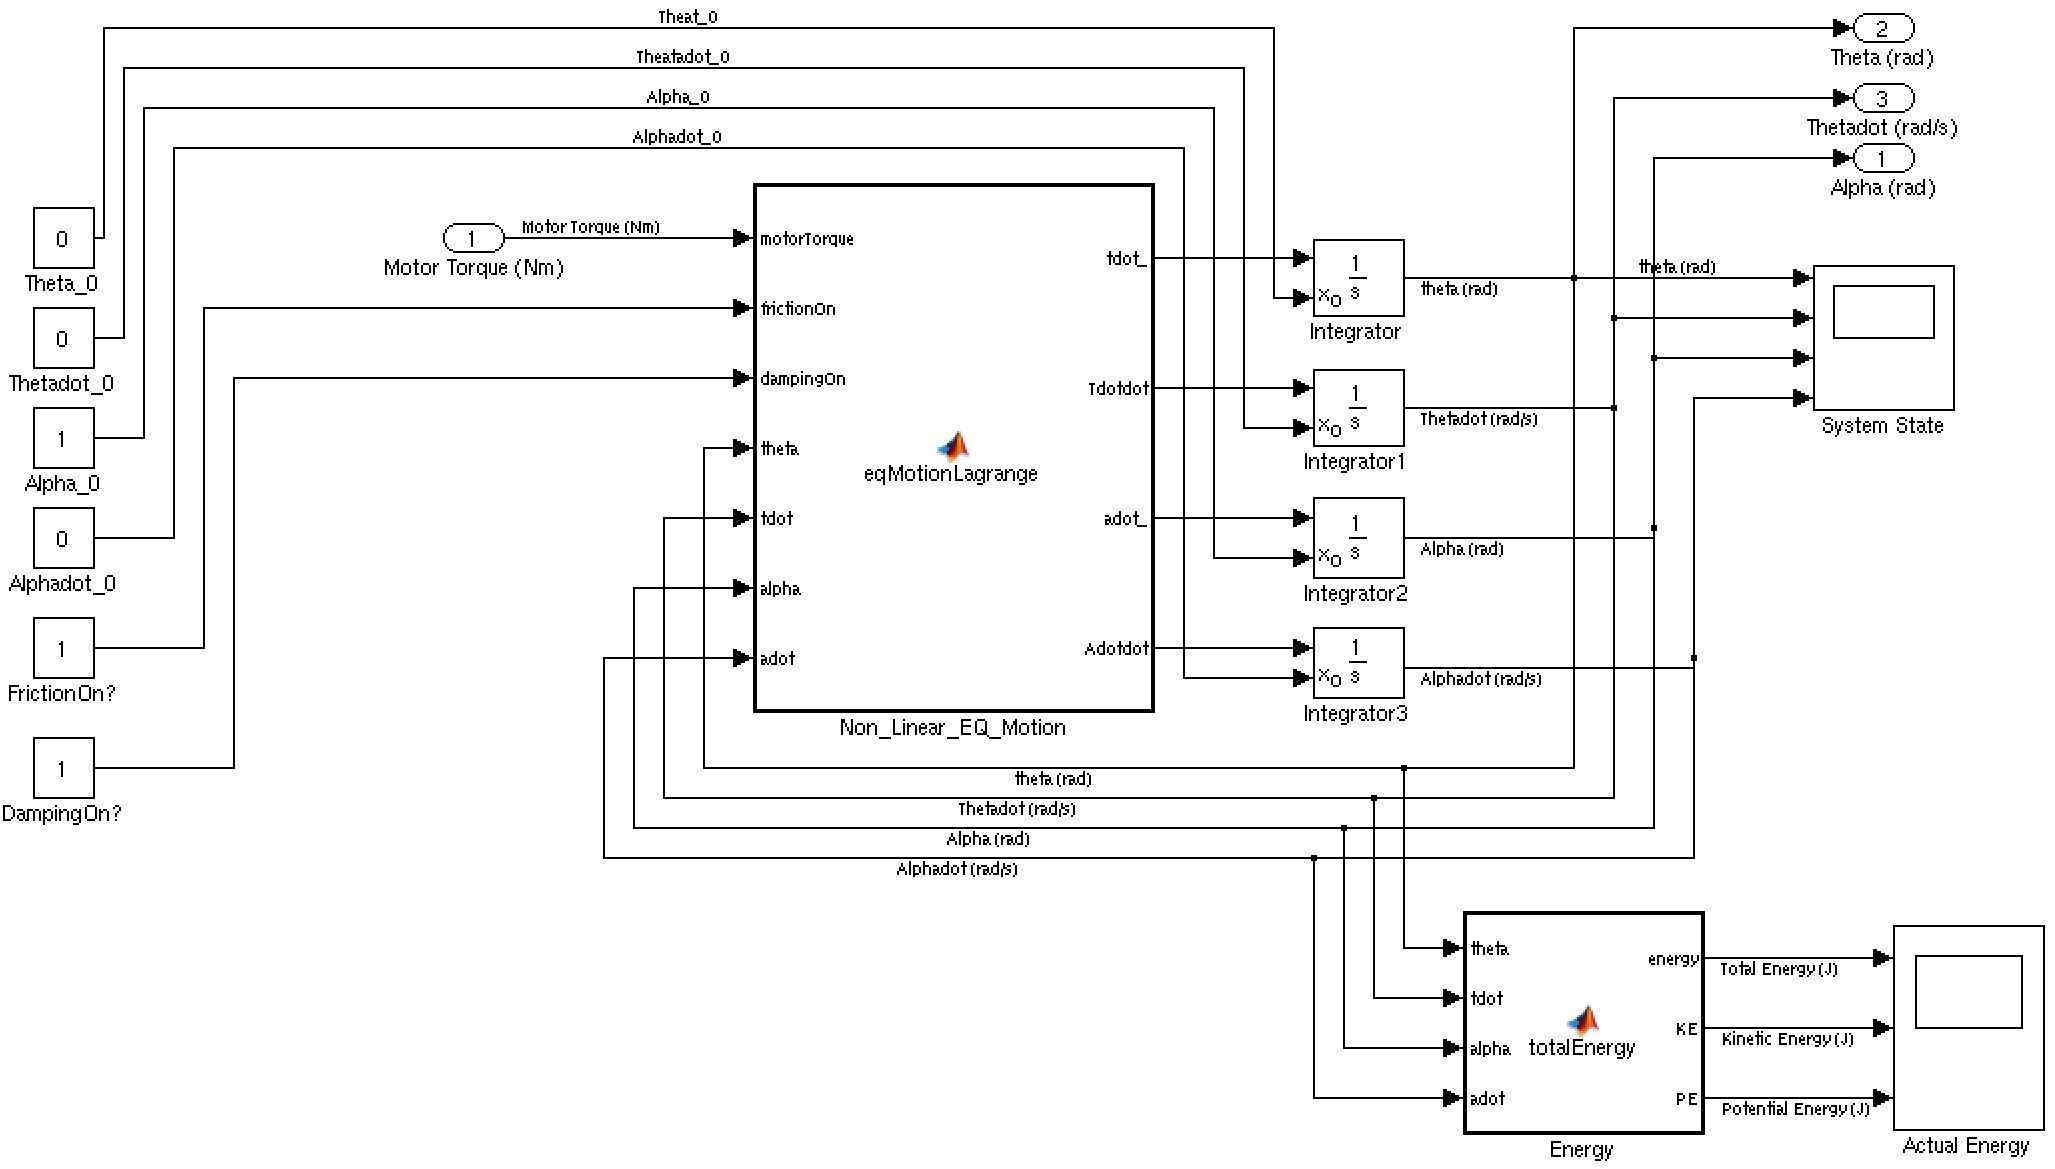
\includegraphics[width = 15cm]{NonLinearModelPic.png}
\end{center}
\caption{Block Diagram of Non-Linear System Model}
\label{NonLinearBlock}
\end{figure}

\begin{figure}
\begin{center}
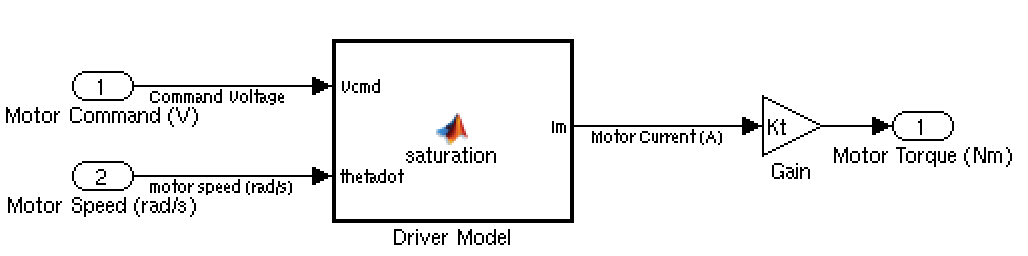
\includegraphics[width = 12cm]{DriverandMotorModel.png}
\end{center}
\caption{Block Diagram of Driver and Electrical Motor Model}
\label{DriverNonLinearBlock}
\end{figure}

\subsection*{e.}
\subsubsection*{Linearized Equations of Motion}

We will linearize the equations of motion about $\theta = 0$, $\alpha = 0$.  By taylor expansion about this point and dropping higher order terms we obtain: 

 $$ \sin(\alpha) \approx 0 \hspace{1cm} \cos(\alpha) \approx \alpha \hspace{1cm} \sin(\theta) \approx 0 \hspace{1cm} \cos{\theta} \approx \theta $$

We note that the coulomb friction terms from the previous non-linear equations must be dropped completely as there is no reasonable linearization of the effects of friction.  We also note that we expect $\dot{\theta}$ and $\dot{\alpha}$ to be relatively small, which implies: 

$$ \dot{\theta} \dot{\alpha} \approx 0 $$

Applying these to equations \eqref{NonLin1} and \eqref{NonLin2} yields \eqref{Lin1} and \eqref{Lin2} respectively.

\begin{equation}
\ddot{\theta} \left( I_{1z1} + I_{2xx} + m_2 l_1^2 \right) + \ddot{\alpha} C_3 = -b_{\theta} \dot{\theta} + \tau_{m}
\label{Lin1}
\end{equation}

\begin{equation}
\ddot{\alpha} C_1 + \ddot{\theta} C_3 - \alpha C_4 = -b_{\alpha} \dot{\alpha} 
\label{Lin2}
\end{equation}

Using equations \eqref{Lin1} and \eqref{Lin2} together we can generate two independent equations for $\ddot{\alpha}$ and $\ddot{\theta}$.

$$ C_{5} = (I_{1z1} + I_{2xx} + m_2 l_1^2) $$

\begin{equation}
\ddot{\theta} = \frac{C_3 b_{\alpha} \dot{\alpha} - C_3 C_4 \alpha - C_1 b_{\theta} \dot{\theta} + C_1 \tau_{m}}{ C_5 C_1 - C_3^2}
\label{Lin_Theta}
\end{equation}

\begin{equation}
\ddot{\alpha} = \frac{-C_5 b_{\alpha} \dot{\alpha}  + C_3 b_{\theta} \dot{\theta}  + \alpha C_4 C_5 - C_3 \tau_m }{C_5 C_1 - C_3^2}
\label{Lin_Alpha}
\end{equation}

\subsubsection*{State Space Model}

State Space Representation models a dynamical system as a set of linear, time-varying differential equations.  What is known as the state of the system is a set of variables, the generalized coordinates, $q_i$ that completely describe the internal state of the system.  For the inverted pendulum we choose the coordinates: 

$$ {\bf{X}}(t) = [q_1(t), q_2(t), q_3(t), q_4(t)]^T = [q_1(t), \dot{q}_1(t), q_3(t), \dot{q}_3(t)]^T = [\theta(t), \dot{\theta}(t), \alpha, \dot{\alpha}(t)]^T $$

In this generalized coordinate system, we compute the derivative of the state, $\dot{X}$ as a function of the current state $\bf{X}$ and the inputs $\bf{u}$. 

$$ \dot{\bf{X}(t)} = [\dot{q}_1(t), \dot{q}_2(t), \dot{q}_3(t), \dot{q}_4(t)]^T = [\dot{q}_1(t), \ddot{q}_1(t), \dot{q}_3(t), \ddot{q}_3(t)]^T = [\dot{\theta}(t), \ddot{\theta}(t), \dot{\alpha}(t), \ddot{\alpha}(t)]^T $$

Because our system is linear this relationship can be related through the State Matrix $A$ and the Input Matrix $B$ which map the current state and external inputs into the system into the change in state through the following equation.

$$ \dot{\bf{X}}(t) = A(t) {\bf{X}(t)} + B(t) {\bf{u}}(t)$$

$$ A_{ij} = \frac{\partial \dot{q}_j}{\partial q_i}(t) \hspace{1cm}  B_{i} = \frac{\partial \dot{q}_i}{\partial u_i}(t)$$

The actual output that we wish to control is determined from $\dot{\bf{X}}(t)$ and from the inputs ${\bf{u}}(t)$ through the Output Matrix, $C(t)$ and the Direct Transmission Matrix $D(t)$.  Then our output ${\bf{Y}}(t)$ can be represented as follows:

$$ {\bf{Y}}(t) = C(t) \dot{\bf{X}}(t) + D(t) {\bf{u}}(t) = C(t) \left\{ A(t) {\bf{X}(t)} + B(t) {\bf{u}}(t) \right\}+ D(t) {\bf{u}}(t)$$

As noted above the matrices A, B, C, and D may in general be functions of time, however because our system is time invariant, these matrices become independent of time.  The notation below has been simplified accordingly.  The matrices A and B may be obtained directly from our linearized equations of motion above.  

\xxx{need to format this matrix to look better}
$$ A = \left[ \begin{array}{c c c c l}
	\frac{\partial \dot{\theta}}{\partial \theta} & \frac{\partial \dot{\theta}}{\partial \dot{\theta}} & \frac{\partial \dot{\theta}}{\partial \alpha} & \frac{\partial \dot{\theta}}{\partial \dot{\alpha}}\\
	\frac{\partial \ddot{\theta}}{\partial \theta} & \frac{\partial \ddot{\theta}}{\partial \dot{\theta}} & \frac{\partial \ddot{\theta}}{\partial \alpha} & \frac{\partial \ddot{\theta}}{\partial \dot{\alpha}}\\
	\frac{\partial \dot{\alpha}}{\partial \theta} & \frac{\partial \dot{\alpha}}{\partial \dot{\theta}} & \frac{\partial \dot{\alpha}}{\partial \alpha} & \frac{\partial \dot{\alpha}}{\partial \dot{\alpha}}\\
	\frac{\partial \ddot{\alpha}}{\partial \theta} & \frac{\partial \ddot{\alpha}}{\partial \dot{\theta}} & \frac{\partial \ddot{\alpha}}{\partial \alpha} & \frac{\partial \ddot{\alpha}}{\partial \dot{\alpha}}\\
 \end{array} \right] = 
\left[ \begin{array}{c c c c l} 
0 & 1 & 0 & 0 \\
0 & \frac{\partial \ddot{\theta}}{\partial \dot{\theta}} & \frac{\partial \ddot{\theta}}{\partial \alpha} & \frac{\partial \ddot{\theta}}{\partial \dot{\alpha}} \\
0 & 0 & 0 & 1 \\
0 & \frac{\partial \ddot{\alpha}}{\partial \dot{\theta}} & \frac{\partial \ddot{\alpha}}{\partial \alpha} & \frac{\partial \ddot{\alpha}}{\partial \dot{\alpha}} \\
\end{array} \right]$$

$$ \frac{\partial \ddot{\theta}}{\partial \ddot{\theta}} = -\frac{C_1 b_{\theta}}{C_5 C_1 - C_3^2}  \hspace{1cm} \frac{\partial \ddot{\theta}}{\partial \alpha} = -\frac{C_3 C_4}{C_5 C_1 - C_3^2}
\hspace{1cm} \frac{\partial \ddot{\theta}}{\partial \dot{\alpha}} = \frac{C_3 b_{\alpha}}{C_5 C_1 - C_3^2}$$

$$ \frac{\partial \ddot{\alpha}}{\partial \dot{\theta}} = \frac{C_3 b_{\theta}}{C_5 C_1 - C_3^2} \hspace{1cm}  \frac{\partial \ddot{\alpha}}{\partial \alpha} = \frac{C_4 C_5}{C_5 C_1 - C_3^2} \hspace{1cm} \frac{\partial \ddot{\alpha}}{\partial \dot{\alpha}} = - \frac{C_5 b_{\alpha}}{C_5 C_1 - C_3^2}$$

$$ B = \left[ \begin{array}{c l} 
\frac{\partial \dot{\theta}}{\partial \tau_m} \\
\frac{\partial \ddot{\theta}}{\partial \tau_m} \\
\frac{\partial \dot{\alpha}}{\partial \tau_m} \\
\frac{\partial \ddot{\alpha}}{\partial \tau_m} \\
 \end{array} \right] 
= \left[  \begin{array}{c l} 
0 \\ \frac{C_1}{C_5 C_1 - C_3^2} \\ 0 \\ -\frac{C_3}{C_5 C_1 - C_3^2} \\
\end{array} \right] $$

We wish to stabilize the pendulum vertically, so the output be are interested in is precisely $\alpha(t)$.  Thus C becomes simply:

$$ C = [0, 0, 1, 0]^T $$

For this system, the only external input, the motor torque $\tau_{m}(t)$, does not directly influence the output, ${\bf{Y}}(t)$ except for its influence on  $\dot{\bf{X}}(t)$ making D simply the zero matrix.

$$ D = [0, 0, 0, 0]^T$$

\subsubsection*{System Transfer Functions}

To generate the transfer functions it is more straight forwards to proceed from equations \eqref{Lin1} and \eqref{Lin2} than from \eqref{Lin_Theta} and \eqref{Lin_Alpha}.  Applying the Laplace transform \eqref{Lin1} and \eqref{Lin2} yields and performing arithmetic operation to isolate $\theta (s)$ and $\alpha (s)$ yields the following transfer functions from motor torque, $ \tau (s)$ to $\theta (s)$ and $\alpha (s)$ respectively.


\begin{equation}
\frac{\theta(s)}{\tau_{m}(s)} = \frac{s^2 C_1 + s b_{\alpha} - C_4}{\left(s^2C_1 + s b_{\alpha} - C_4 \right) \left(s^2 C_5  + s b_{\theta} \right) - s^4 C_3^2}
\label{TF_Theta}
\end{equation}

\begin{equation}
\frac{\alpha(s)}{\tau_{m}(s)} = \frac{-s^2 C_3}{\left(s^2C_1 + s b_{\alpha} - C_4 \right) \left(s^2 C_5  + s b_{\theta} \right) - s^4 C_3^2}
\label{TF_Alpha}
\end{equation}

If we were to neglect the effects of damping, then \eqref{TF_Theta} and \eqref{TF_Alpha} would reduce to the following:

$$ \frac{\theta(s)}{\tau_{m}(s)} \approx \frac{s^2 C_1 - C_4}{s^2 \left[s^2 \left(C_5 C_1 - C_3^3 \right) - C_4 C_5\right]} $$

$$ \frac{\alpha(s)}{\tau_{m}(s)} \approx \frac{- s^2 C_3}{s^2 \left[s^2 \left(C_5 C_1 - C_3^3 \right) - C_4 C_5\right]} $$

In the simplified transfer function for $\alpha (s)$ above it appears as if we can cancel the but this not the case as we see when we examine equation \eqref{TF_Alpha}.  

\section*{2. Parameter Identification}
The inverted pendulum system includes many parameters related to the mechanical and electrical properties of the system. To determine these, we used a combination of manufacturer data sheets, CAD modeling, physical measurements, and experimental regression.\\

Most of the relevant motor parameters were previously determined in the DC motor lab. In that case, most of the parameters were provided by the manufacturer, but we performed regression on experimental data to fit our model with the test data and found that the true values were different from those on the data sheet. The relevant values are shown in table \ref{q2_1}. An abbreviated except from our DC motor lab is given below to show our procedure for determining these values. \\

\begin{table}[htb]
\begin{center}
    \begin{tabular}{|c|c|c|}
        \hline
        ~                 & Data-Sheet Values    & Fit Values              \\ \hline
        $J_{motor} \hspace{0.1cm} \left( \frac{N \cdot s^2}{m} \right)$               & $8.5 \cdot 10^{-6} $     & $3.50514 \cdot 10^{-5}$ \\ 
        $K_{t} \hspace{0.1cm} \left( \frac{N\cdot m}{A} \right)$           & $0.0424$             & $0.0314499$             \\ 
        $b_{forwards} \hspace{0.1cm} \left( N \cdot s \right)$    & $3.7 \cdot 10^{-6} $ & $1.08586 \cdot 10^{-5}$ \\ 
        $b_{reverse} \hspace{0.1cm} \left( N \cdot s \right)$     & $3.7 \cdot 10^{-6} $ & $4.85930 \cdot 10^{-5}$ \\ 
        $\tau_{forwards} \hspace{0.1cm} \left( N \cdot m \right)$ & $5.6 \cdot 10^{-3}$  & $0.0224389$             \\ 
        $\tau_{reverse} \hspace{0.1cm} \left( N \cdot m \right)$   & $5.6 \cdot 10^{-3}$  & $0.0143096$             \\
        \hline
    \end{tabular}
\caption{DC Motor Final Parameter Values vs Original Data Sheet Values}
\label{q2_1}
\end{center}
\end{table}

To determine the parameters of the motor we used MATLAB's numerical differential equation solving to simulate the trajectory of the system as a function of time, driver current, $I_t$ and our unknown system parameters $J$, $b$, $K_t$, and $\tau_{coulomb}$.  By then
comparing the predicted angular positions with the measured angular positions over time, we can construct a non-linear regression to estimate the unknown parameters.  We collected a data set where the driver was given a sinusoidal voltage, and we assume that motor current, $I_m$, is identical to this driver voltage and recorded the motor motion that this input caused. \\

With this model and some intelligent guessing for new parameter values, we arrived at an excellent fit shown in figure \ref{q2_2}. The most notable feature of these values is the large difference between the torque of friction in the forwards and reverse directions. \\ 

\begin{figure}[htb]
\begin{center}
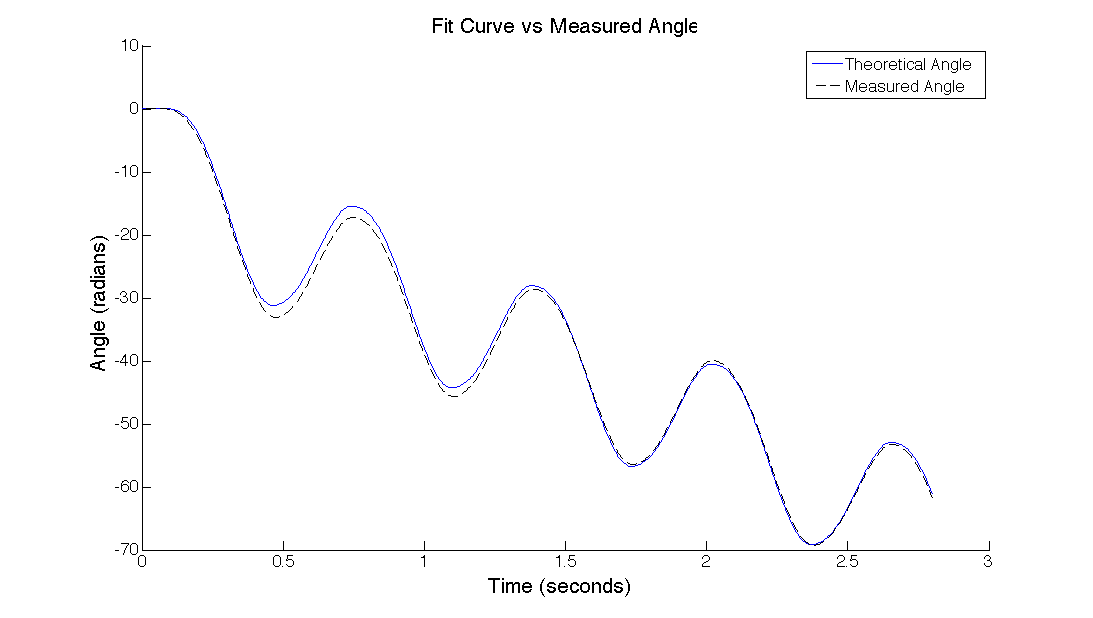
\includegraphics[width = 14cm]{awesomefitFiner.png}
\caption{Predicted behavior vs Actual behavior using fit parameter values and enhanced modeling}
\label{q2_2}
\end{center}
\end{figure}

With the motor parameters largely known already, we focused on determining the parameters of the new components comprising the pendulum and horizontal arm. To ensure accuracy, we used multiple methods and compared results. For example, all of the mass of every component was determined on the scale provided in the mechatronics lab. We then built CAD models of every component in SolidWorks using a combination of engineering drawings, physical measurements, and already built models from McMaster-Carr. By setting the material properties correctly, SolidWorks can determine the mass of every part. We compared this calculated value to the measured values and they all matched within the limits of resolution of the scale. This gave us confidence in the ability of SolidWorks to calculate the other necessary parameters.Therefore, we built assemblies of the pendulum, the horizontal arm and complete system, and we used SolidWorks to calculate the masses, centers of mass, and moments of inertia that we needed. Figures \ref{q2_3}, \ref{q2_4}, and \ref{q2_5} show the CAD assemblies. The inertia matrix for the pendulum and other relevant values are given below. Note that the axes labels in the SolidWorks models are not the same as those in our derived equations.

\begin{center} $ \begin{vmatrix}
\bar{I}_{xx} & \bar{I}_{xy} & \bar{I}_{xz} \\
\bar{I}_{yx} & \bar{I}_{yy} & \bar{I}_{yz} \\
\bar{I}_{zx} & \bar{I}_{zy} &  \bar{I}_{zz} \end{vmatrix}_{Pendulum}
=  \begin{vmatrix}
8.1\cdot10^{-6} & 2.03\cdot10^{-5} & 0 \\
2.03\cdot10^{-5} & 3.711\cdot10^{-4} & 0 \\
0 & 0 &  3.646\cdot10^{-4} \end{vmatrix}$\end{center}

Translating from the coordinate system established in Solid Works to our coordinate system yields the following moment of inertia tensor:

$$I_{2} = \left[ \begin{array}{c c c l} 
8.1\e{-6} & 0 & 2.03\e{-5} \\   
0 & 3.711\e{-4} & 0 \\
2.03\e{-5} & 0 & 3.646e{-4} \\
\end{array} \right] \, kg \cdot m^2$$

\begin{center}
$$m_{1} = 0.1481 kg \quad m_{2} = 0.0820 kg $$
$$ l_{1} = 0.10826 m \quad l_{2C} = 0.08568 m $$
$$I_{1zt} = \left(6.78 \e{-4} + 3.50514 \e{-5} \right) \, kg \cdot m^2 =  7.1305\cdot 10^{-4}kg\cdot m^{2}$$
\end{center}

\begin{figure}[htb]
\begin{center}
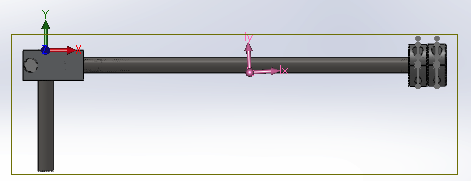
\includegraphics[width = 14cm]{Pendulum.png}
\caption{SolidWorks Model of Pendulum}
\label{q2_3}
\end{center}
\end{figure}

\begin{figure}[htb]
\begin{center}
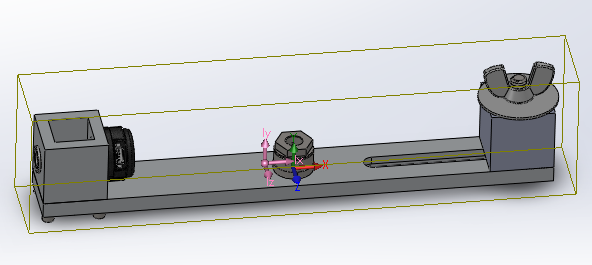
\includegraphics[width = 14cm]{Horizontal.png}
\caption{SolidWorks Model of Horizontal Link}
\label{q2_4}
\end{center}
\end{figure}

\begin{figure}[htb]
\begin{center}
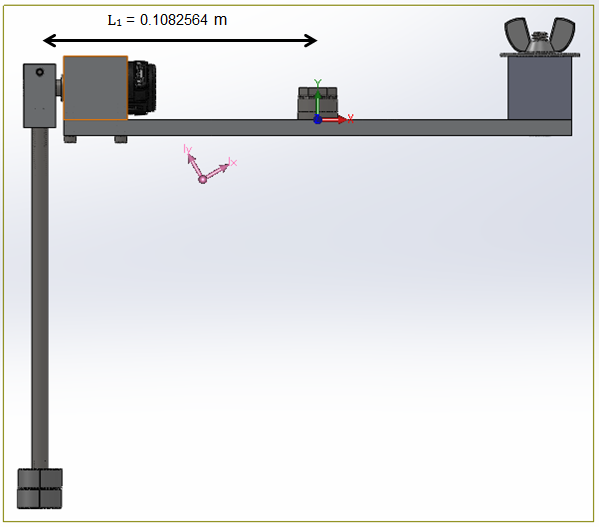
\includegraphics[width = 14cm]{CompleteArm.png}
\caption{SolidWorks Model of Assembled Pendulum and Horizontal Link}
\label{q2_5}
\end{center}
\end{figure}

For the pendulum we assume that frictional torque, $\tau_{F \alpha}$, and the viscous damping coefficient, $b_{\alpha}$ to be the same in each direction. These terms for the pendulum were estimated in an experiment where the horizontal arm was fixed in place and the pendulum was allowed to swing freely from an initial angle.  By comparing the decaying envelope, extracted as the maximum and minimum of each oscillation, of the actual system motion with a similar plot generated from a simulated model, we formed a rough estimate of these terms. 

%To determine the viscous damping and coulomb friction of the pendulum and bearings, we used non-linear regression with MATLAB's numerical differential equation solver, just as we did with the DC motor parameter identification. To do this we clamped the horizontal arm in place and allowed the pendulum to oscillate freely from several starting positions. Because of the large number of data points obtained during the time it takes the pendulum to come to rest, we extracted the peak of each oscillation for the regression instead of using every point. The damping and friction values are given below; because the friction and damping in the pendulum and bearings are so small, we assumed that they were approximately equal in both directions.\\
$$b_{\alpha} = 6.5\cdot10^{-6}\, N\cdot s \qquad \tau_{F \alpha} = 7.0\cdot10^{-6} \, N\cdot m$$

\begin{figure}
\begin{center}
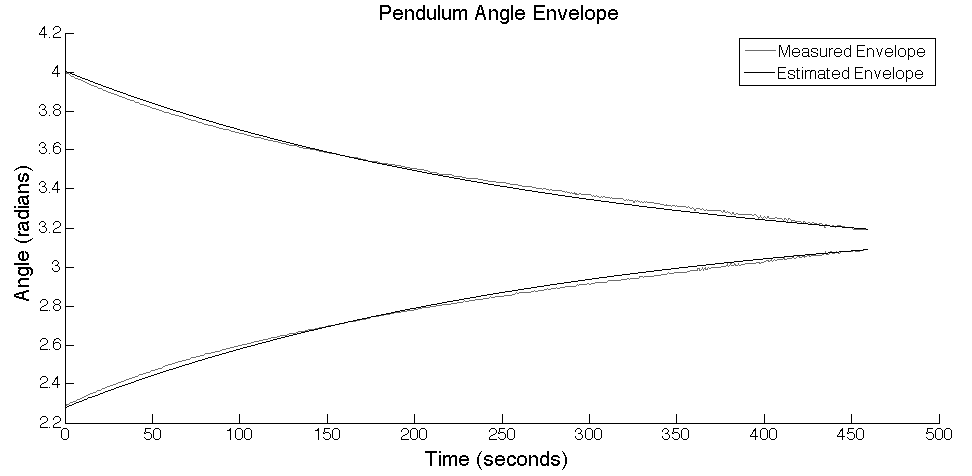
\includegraphics[width = 16cm]{pendulumEnvelope.png}
\end{center}
\label{Actual Decaying Envelope of motion vs Simulated Envelope}
\end{figure}


\section*{3. Comparing Linear and Non-Linear Models}

\section*{4. State Space Controls in Simulink}

\section*{5. Swing Up Controller in Simulink}

\section*{6. LabView Implementation}

\subsection*{a.}

\subsection*{b.}

\subsection*{c.}

\subsection*{d.}

\section*{7. Effects on LabView Loop Rate on Stability}

\section*{8. Classical Controller}

\section*{9. Another Swing Up Controller}

\section*{10. Parasitic Effects}

\section*{Appendix.}

\xxx{Add matlab code and stuff here}

\end{document}